This section includes Alloy code that describes the model and checks wether it is consistent or not.
At the of the code, Class Diagram and Alloy generated World are shown.

\myparagraph{Alloy Code}
% Settings for Alloy code listing.
\lstset{
    language=alloy,
    numbers=left,
    numberstyle=\tiny,
    stepnumber=2,
    tabsize=4,
    keywordstyle=\color{alloy-keyword}\bfseries,
    commentstyle=\color{alloy-comment},
    stringstyle=\color{alloy-string},
    basicstyle=\small\fontfamily{pcr}\selectfont, % Courier font family
}

% Includes the Alloy model file.
\lstinputlisting{./files/Alloy.als}
\vfill

\begin{figure}[H]
  \begin{center}
  	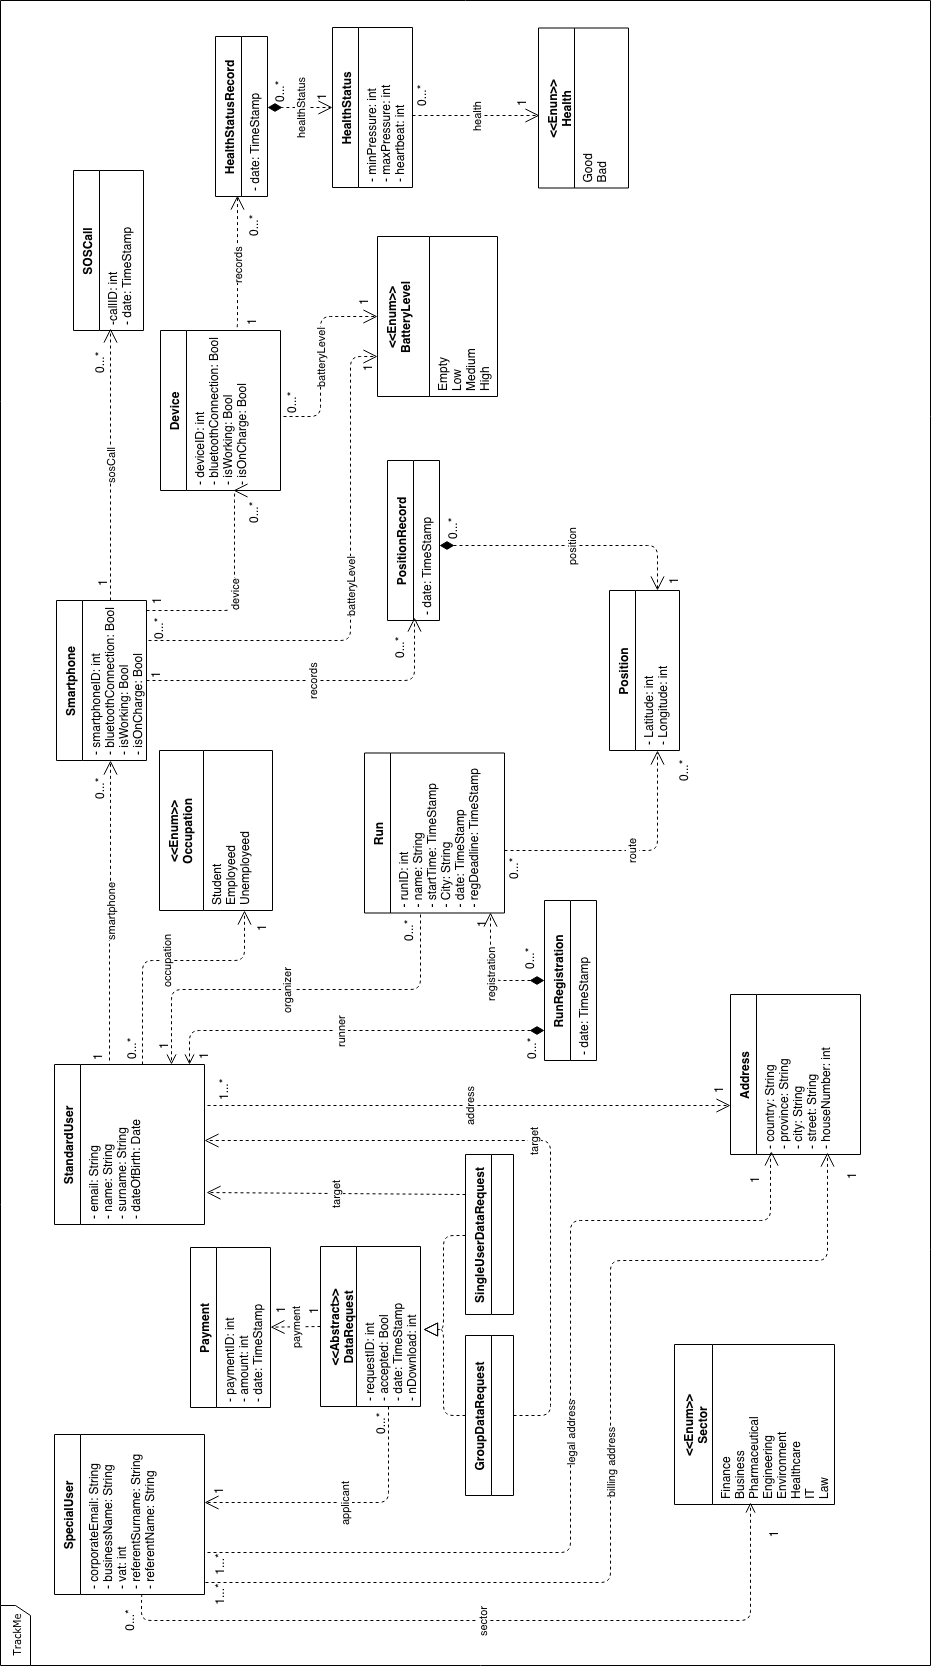
\includegraphics[height=0.68\paperheight]{./img/Class_Diagram.png}
		\caption{\textit{Class diagram} of the structure of the system-to-be.}
    \hspace{0.05\linewidth}
    \centering
		\label{classDiagram}
    \end{center}
\end{figure}
